\documentclass[preprint, 3p,
authoryear]{elsarticle} %review=doublespace preprint=single 5p=2 column
%%% Begin My package additions %%%%%%%%%%%%%%%%%%%

\usepackage[hyphens]{url}

  \journal{Transport Geography?} % Sets Journal name

\usepackage{graphicx}
%%%%%%%%%%%%%%%% end my additions to header

\usepackage[T1]{fontenc}
\usepackage{lmodern}
\usepackage{amssymb,amsmath}
% TODO: Currently lineno needs to be loaded after amsmath because of conflict
% https://github.com/latex-lineno/lineno/issues/5
\usepackage{lineno} % add
\usepackage{ifxetex,ifluatex}
\usepackage{fixltx2e} % provides \textsubscript
% use upquote if available, for straight quotes in verbatim environments
\IfFileExists{upquote.sty}{\usepackage{upquote}}{}
\ifnum 0\ifxetex 1\fi\ifluatex 1\fi=0 % if pdftex
  \usepackage[utf8]{inputenc}
\else % if luatex or xelatex
  \usepackage{fontspec}
  \ifxetex
    \usepackage{xltxtra,xunicode}
  \fi
  \defaultfontfeatures{Mapping=tex-text,Scale=MatchLowercase}
  \newcommand{\euro}{€}
\fi
% use microtype if available
\IfFileExists{microtype.sty}{\usepackage{microtype}}{}
\usepackage[]{natbib}
\bibliographystyle{plainnat}

\usepackage{graphicx}
\ifxetex
  \usepackage[setpagesize=false, % page size defined by xetex
              unicode=false, % unicode breaks when used with xetex
              xetex]{hyperref}
\else
  \usepackage[unicode=true]{hyperref}
\fi
\hypersetup{breaklinks=true,
            bookmarks=true,
            pdfauthor={},
            pdftitle={Leveraging GTFS to explore spatial patterns in transit supply with respect to social needs},
            colorlinks=false,
            urlcolor=blue,
            linkcolor=magenta,
            pdfborder={0 0 0}}

\setcounter{secnumdepth}{5}
% Pandoc toggle for numbering sections (defaults to be off)


% tightlist command for lists without linebreak
\providecommand{\tightlist}{%
  \setlength{\itemsep}{0pt}\setlength{\parskip}{0pt}}




\usepackage{subfig}
\usepackage{booktabs}
\usepackage{longtable}
\usepackage{array}
\usepackage{multirow}
\usepackage{wrapfig}
\usepackage{float}
\usepackage{colortbl}
\usepackage{pdflscape}
\usepackage{tabu}
\usepackage{threeparttable}
\usepackage{threeparttablex}
\usepackage[normalem]{ulem}
\usepackage{makecell}
\usepackage{xcolor}



\begin{document}


\begin{frontmatter}

  \title{Leveraging GTFS to explore spatial patterns in transit supply
with respect to social needs}
    \author[Public Transport Research Group (PTRG)]{James Reynolds%
  %
  \fnref{1}}
   \ead{james.reynolds@monash.edu} 
    \author[Public Transport Research Group (PTRG)]{Yanda Qu%
  %
  \fnref{2}}
   \ead{yanda.qu@monash.edu} 
    \author[Public Transport Research Group (PTRG)]{Graham Currie%
  \corref{cor1}%
  \fnref{3}}
   \ead{graham.currie@monash.edu} 
      \affiliation[Public Transport Research Group (PTRG)]{
    organization={Public Transport Research Group (PTRG), Institute of
Transport Studies, Department of Civil Engineering Engineering, Monash
University},addressline={Clayton
Campus},city={Melbourne},postcode={3800},state={Victoria},country={Australia},}
    \cortext[cor1]{Corresponding author}
    \fntext[1]{Research Fellow}
    \fntext[2]{PhD Student}
    \fntext[3]{Professor}
  
  \begin{abstract}
  This is the abstract.

  It consists of two paragraphs.
  \end{abstract}
    \begin{keyword}
    keyword1 \sep 
    keyword2
  \end{keyword}
  
 \end{frontmatter}

\section{Introduction}\label{introduction}

Approaches for assessing spatial gaps between social needs for transport
and what transit is supplied have been reported in previous research,
including in \citet{Currie2003Hobart}, \citet{Currie2004Gap},
\citet{Currie2007Identifying} and \citet{currie2010identifying}. These
publications presented a transit Supply Index (SI) and used to identify
geographic areas in a few Australian cities where there were very high
social needs for transport, but very little transit service, or no
transit at all. This approach suggested a new way for transit planners
to identify and prioritise locations, targetted towards improving
mobility for populations who might not have sufficient mobility to meet
their basic needs or fully participate in society.

However, in almost two decades since the SI was developed there does not
appear to have been much further use of this approach. It is also
unclear whether gaps between social needs and transit supply have
increased or reduced in Australian cities; or if the spatial patterns
identified in Hobart \citep{Currie2003Hobart, Currie2004Gap} and
Melbourne \citep{Currie2007Identifying, currie2010identifying}, are
similar in other places This may in part be because applying such
methodologies elsewhere would, at the time, appear likely to have
required a bespoke data collection, cleaning and analysis effort.
Transit timetables were typically publicly available in paper and/or PDF
formats, while the analyses reported in \citet{Currie2003Hobart},
\citet{Currie2004Gap}, \citet{Currie2007Identifying} and
\citet{currie2010identifying} appear to have been mostly based on
special data provided directly to the research by transit operators and
authorities in each location.

Nowadays, the General Transit Feed Specification (GTFS) allows timetable
data to be published in a standardized format. More than 10,000 transit
agencies publically release data this way. Various tools for maniulating
GTFS data are now available, including validation, analysis and
visualization tools. As GTFS data is typically published online, free to
the user, and without usage restrictions, it appears widely used in
transport research and practice, and amongst actors in the technology
sectors, notably to provide transit directions on the Google Maps
platform, being the use case for which it was originally developed
\citep{GTFS}.

However, the availability of tools that might be used by researchers,
practitioners and advocates use GTFS data to examine spatial patterns in
transit supply and social needs for transport appears limited.\\
This gap and the lack of direct follow up to \citet{Currie2003Hobart},
\citet{Currie2004Gap}, \citet{Currie2007Identifying} and
\citet{currie2010identifying} provide the motivation for the research
reported in this paper.\\
The research included the developement of a new R package
(gtfssupplyindex) that can be used to calculate SI scores Also presented
in this paper are results for Greater Melbourne in 2016 and 2021,
matching the most recent censuses, that are comparable\\
to the 2006 results reported in \citet{currie2010identifying}.
Comparisons are also made to other parts of Australia, so as to explore
whether findings about Greater Melbourne are generalizable.

The remainder of this paper is structured as follows: the next section
outlines the background to this research, including the formulation of
the Transit Supply Index (SI) and an explanation of the GTFS. Section 3
then describes the study methodology, followed by presentation of
results in Section 4. Section 5 discusses the findings. Limitations of
this study, directions for future research and a brief conclusion are
provided in Section 6.

\section{Background}\label{background}

\subsection{Transit metrics}\label{transit-metrics}

Even a brief search reveals many metrics available for benchmarking
transit services. Examples include: those in the extensive Transit
Cooperative Research Program (TCRP) Report 88 guidebook on developing
performance-measurement systems \citep{Ryus:2003aa}; those used across
benchmarking databases and programs
\citep{Florida-Transit-Information-System:2018aa, UITP:2015aa, Imperial-College-London:2023aa};
and the Transit Score website \citep{WalkScore:2023tg}. The Fielding
Triangle \citep{FieldingGordonJ1987Mpts} provides a framework for
combining indicators of service inputs, outputs and consumption to
describe cost efficiency, cost effectiveness and service effectiveness.
More broadly: \citet{Litman:2003ab} and \citet{Litman:2016aa} discuss
some of the traffic, mobility, accessibility, social equity, strategic
planning and other rational decision-making-based perspectives underling
transport indicators; \citet{Reynolds:2017ah} extends these into models
of how institutionalism, incrementalism and other public policy analysis
concepts might apply to decision-making processes relating to transit
prioritization; \citet{GuzmanLuisA.2017Aeit}\\
developed a measure of accessibility in the context of policy
development and social equity for Latin American Bus Rapid Transit (BRT)
networks; and \citet{Creutzig2020streetspaceallocation} introduced
street space allocation metrics based around ten ethical principles.

However, many such metrics may be difficult to calculate, explain or
understand, especially for those who are not planners, engineers or
other technical specialists. Where pre-calculated transit metrics are
immediately available, such as on a website or other online platform, it
may not be possible for practitioners, researchers or advocates to
independently generate scores, for instance to assess proposed system
changes.

Contrasting examples are provided by the metrics in the TCQSM and the
Transit Score metric \citep{WalkScore:2023tg}. Transit Scores are
readily available on the Transit Score website for locations with a
published GTFS feed. The meaning of these Transit Scores also appears
easy to explain, with the highest possible score of 100 representing the
sort of transit accessibility that might be xperienced in the center of
New York. However, the Transit Score algorithm is a black box, and
scores cannot be calculated independently or generated for proposed
changes to networks. In contrast, the TCQSM provides a wide range of
metrics for measuring different aspects of a transit system. The TCQSM
scores themselves appear easy to understand or explain, ranging from A
(good) to F (bad), although the large number of metrics might be
somewhat overwhelming for some users. The scores, however, can be
calculated independently, given sufficient data. \citet{Wong:2013aa}
provides an example of what can be done with GTFS data, open metrics and
coding by reporting the distribution of various TCQSM metrics across 50
USA transit operators.

\subsection{The Transit Suppy Index}\label{the-transit-suppy-index}

A generalized form of the SI equation, adapted from
\citet{currie2010identifying}, is:

\[SI_{area, time} = \sum{\frac{Area_{Bn}}{Area_{area}}*SL_{n, time}}\]

where:

\begin{itemize}
\item
  \(SI_{area, time}\) is the Supply Index for the area of interest and a
  given period of time;
\item
  \(Area_{Bn}\) is the buffer area for each stop (n) within the area of
  interest (in \citet{currie2010identifying} this was based on a radius
  of 400 metres for bus and tram stops, and 800 metres for railway
  stations);
\item
  \(Area_{area}\) is the area of the area of interest; and
\item
  \(SL_{n,time}\) is the number of transit arrivals for each stop for a
  given time period.
\end{itemize}

\begin{figure}
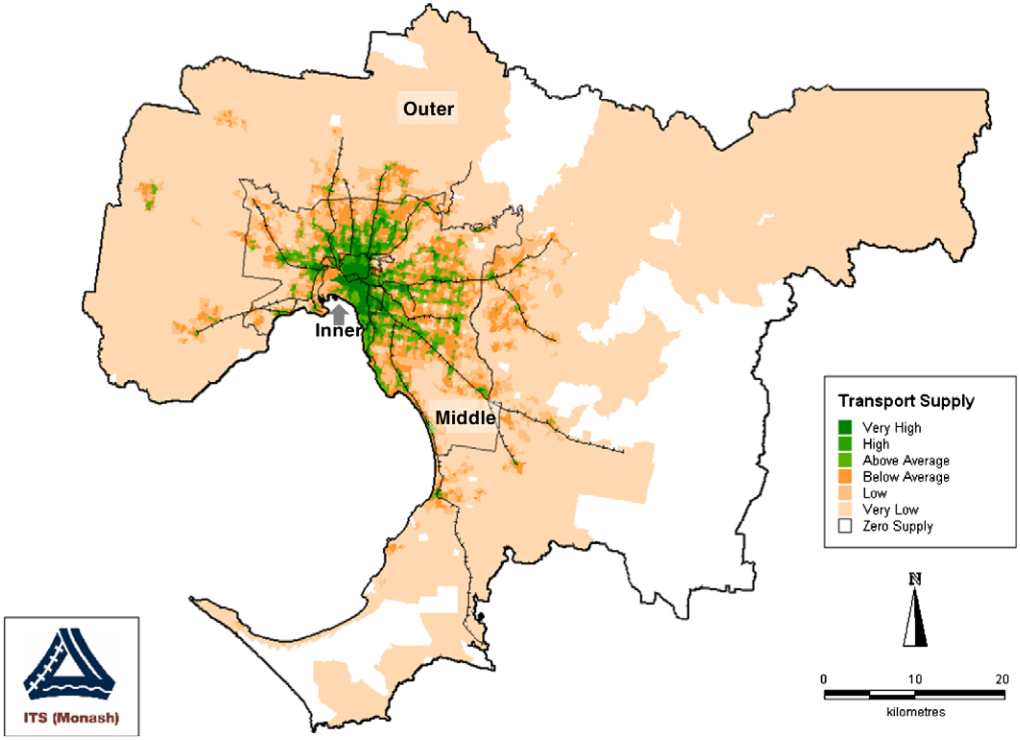
\includegraphics[width=1\linewidth]{graphics/Currie2010SI} \caption{Distribution of supply measure scores – Metropolitan Melbourne (2006), Source: Currie (2010)}\label{fig:Currie_map_SI}
\end{figure}

\citet{currie2010identifying} reported SI scores across Greater
Melbourne in 2006, as shown in Figure \ref{fig:Currie_map_SI}. The
general patterns appear to be higher levels of transit supply in the
middle and inner suburbs and along passenger railway lines. Outer areas
tend to have very low SI scores or no transit supply at all.

\subsection{Social need and needs gap}\label{social-need-and-needs-gap}

As well as measuring transit supply, \citet{currie2010identifying} also
assessed the social need for transit across Greater Melbourne using: the
Australian Bureaus of Statistics' Index of Related Socio-Economic
Advantage/Disadvantage (IRSAD); a transport needs index derived by
\citet{currie2010identifying} from eight weighted indicators; and a
combination of the two. Figure \ref{fig:Currie_map_gap} reproduces the
resultant map identifying areas with very high transport needs, but very
low or no transit supply.

\begin{figure}
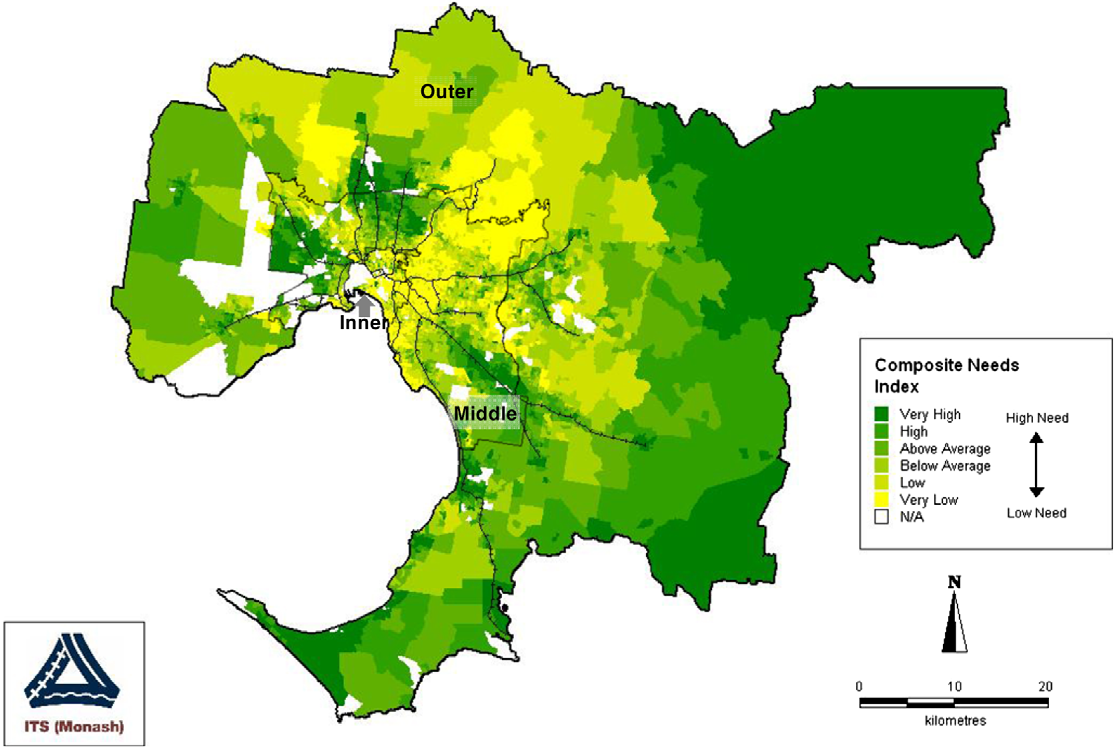
\includegraphics[width=1\linewidth]{graphics/Currie2010Needs} \caption{Distribution of categories of composite social need index scores, Source: Currie (2010)}\label{fig:Currie_map_needs}
\end{figure}

\begin{figure}
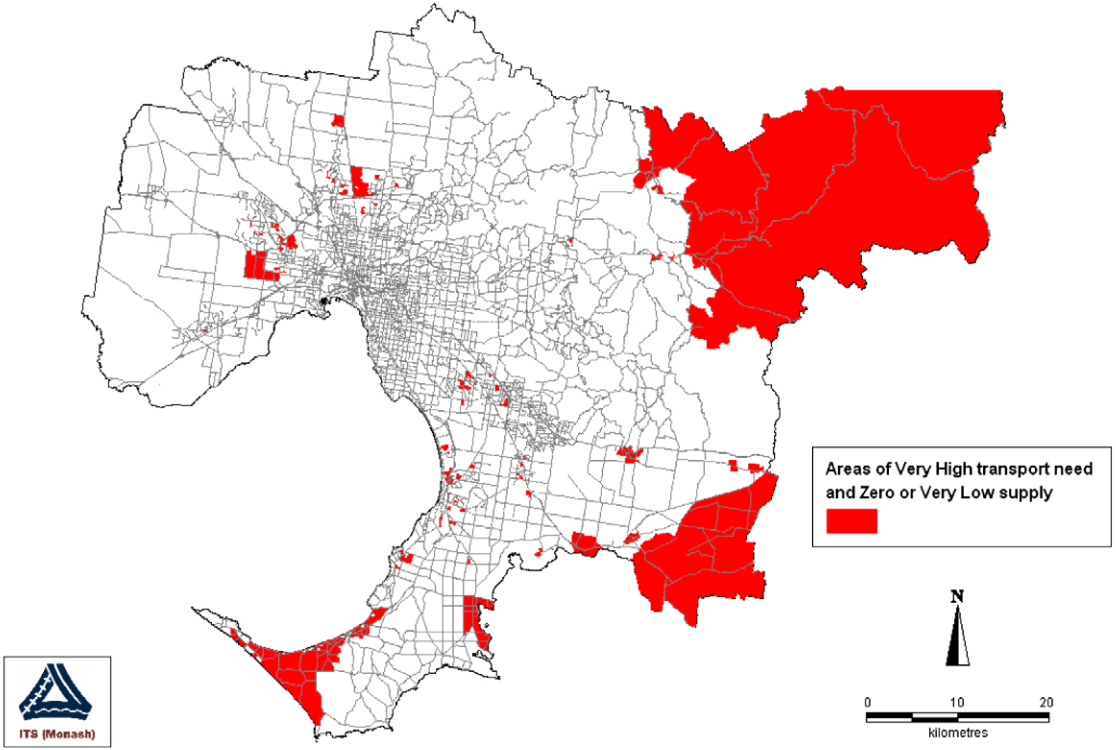
\includegraphics[width=1\linewidth]{graphics/Currie2010gap} \caption{Melbourne needs-gap – very high transport need areas with zero or very low public transport supply, Source: Currie (2010)}\label{fig:Currie_map_gap}
\end{figure}

The results indicated various areas where service gaps might be of
concern, especially in outer parts of Melbourne where low density
development patterns make provision of transit more challenging.
\citet{currie2010identifying} found that ``(o)verall, 8.2\% of Melbourne
residents have `very high' needs but `zero', `low' or `very low' public
transport supply.''\\
They also suggested that planning for transit service provision using
this approach would be ``substantially more useful than the presentation
of anecdotal evidence, which is the most common means of identifying
transport needs in local transport studies throughout the world.''
However, it doesn't appear that this approach has been widely adopted in
practice or academia. Our suspicion is that while the SI has a
relatively simple formula and requires only geographic and timetable
data, the lack of a software tool to perform these calculations may be
part of the reason that it has not been more widely adopted and why
formal needs-supply-gap analysis may still be uncommon.

It is also unclear whether the patterns in Melbourne identified in
\citet{currie2010identifying}, where areas with very high transport
needs but zero or very low transit supply tend to be in outer areas
serviced by buses, are similar to patterns in other cities. Nor is it
clear whether the patterns in Melbourne itself have changed since the
2006 analysis. Developing a software tool to calculate SI tools from
GTFS data, and then using it to comparing current conditions and other
locations to the findings of \citet{currie2010identifying}, therefore,
is the primary aim of this paper.

\section{Methodology}\label{methodology}

\subsection{Transit Supply Index}\label{transit-supply-index}

This study developed a package of tools for calculating the SI from GTFS
data using the R programming language \citep{R-base}. The
recommendations of \citet{wickham2023r} informed the package setup and
development approach. Various existing packages were relied upon
including: the sf package \citep{R-sf} for geospatial analysis; the
tidyverse \citep{tidyverse2019}; gtfstools \citep{R-gtfstools}; and
tidytransit \citep{R-tidytransit}. Australian Bureau of Statistics (ABS)
data was also used, sourced via the strayr and absmapsdata packages
\citep{r-strayr}. Some code was adapted from examples, vignettes and
other documentation in these and other packages.

Two cases were used during the code development and testing, such that
results might be generated for real GTFS data: the Mornington Peninsula
Tourist Railway GTFS feed; and the Public Transport Victoria (PTV) GTFS
feed, both in Victoria, Australia. Both were selected primarily for
convenience, given that the authors are familiar with the typical
service patterns and geography. Adopting the Mornington Peninsula
Tourist Railway network, which consists of only three stations, also
facilitated hand calculation of the SI as a cross-check of the results
produced by the developed package.

Figure @ref(Melbourne\_map)) shows the areas of interest relevant to the
code development and testing, and selected railway stations. Statistical
Area (SA) zones were adopted from the Australian Bureau of Statistics
\citep{ABSmaps} as the areas of interest, and included SA3
zones\footnote{These are generally similar to Local Government Area
  (LGA) boundaries.} across the Greater Melbourne Greater Capital City
statistical area (Figure @ref(Melbourne\_map), left); and SA1
zones\footnote{SA1 zones are the smallest geographical areas for which
  results are reported in the Australian census.} within 800 metres of
the Mornington Penninsula railway (Figure @ref(Melbourne\_map), right).

\begin{figure}
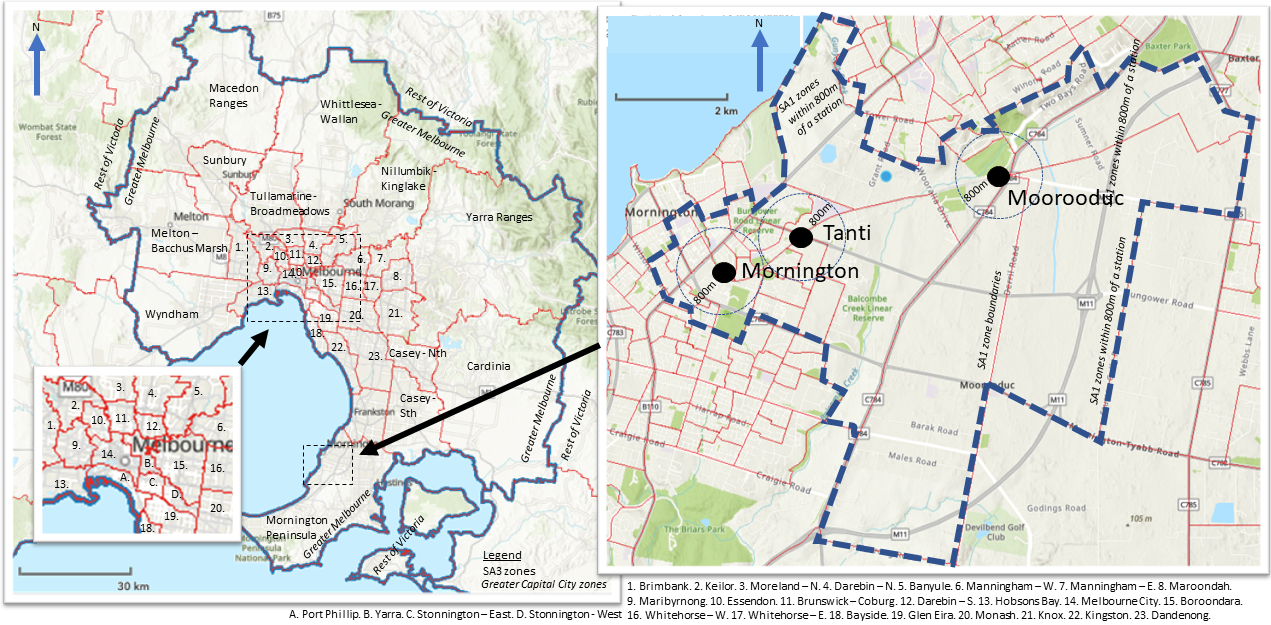
\includegraphics[width=1\linewidth]{graphics/all_maps} \caption{Areas of interest}\label{fig:Melbourne_map}
\end{figure}

\subsubsection{Mornington Penninsula Tourist
Railway}\label{mornington-penninsula-tourist-railway}

The Morning Peninsula Tourist Railway is in the outer south-east of
Melbourne, running on Sundays and Wednesdays between Mornington and
Moorooduc, with an intermediate stop at Tanti Park\footnote{see
  https://transitfeeds.com/p/mornington-railway/806/latest/stops}. A
GTFS feed from 2018 was selected for the purposes of tests, and for
demonstrating the code and outputs reported here.

\subsubsection{Public Transport Victoria
(PTV)}\label{public-transport-victoria-ptv}

The Victorian GTFS feed, published by Public Transport Victoria (PTV)
and with historical feeds sourced via
\citet{transitfeeds_victoria:2023aa}, was used for analysis of Greater
Melbourne and Victoria. SI scores were obtained for the weeks starting
on the day of the census in 2016 and 2021, which were on Tuesday 9th and
10th of August respectively.

\subsubsection{Australian Capital
Territory}\label{australian-capital-territory}

\subsubsection{Adelaide}\label{adelaide}

\subsubsection{Metro Tasmania Burnie}\label{metro-tasmania-burnie}

\subsubsection{Metro Tasmania Hobart}\label{metro-tasmania-hobart}

\subsubsection{Metro Tasmania
Launceston}\label{metro-tasmania-launceston}

\subsubsection{Translink South East
Queensland}\label{translink-south-east-queensland}

\subsubsection{Transperth}\label{transperth}

\subsection{Measuring social
disadvantage}\label{measuring-social-disadvantage}

This study adopts the same approach to measuring social disadvantage as
\citet{currie2010identifying}, using: the Australian Bureau of
Statistics Index of Relative Socio-Economic Advantage/Disadvantage
(IRSAD); and a transport needs index, which included the same need
indicators and weightings as used in
\citet{currie2010identifying}\footnote{Indicators: Adults without cars
  (weighting 0.19); accessibility (distance to Central Buisness
  District, 0.15); persons aged over 60 years (0.14); persons on a
  disability pension (0.12); low income families (0.10); adults not in
  the labour force (0.09); students (0.09); and persons aged 5-9 years
  (0.12). Data was extracted from the 2021 census, including the
  disability pension data which is now available through the ABS rather
  than Centrelink. A income of \$799 or lower per week was adopted as
  the threshold for low income households, based on updating the \$499
  figure used in \citet{currie2010identifying} to account for inflation,
  using the Reserve Bank of Australia's online inflation calculator.
  Note also that the 2021 census reported low-income families rather
  than households, as was used in \citet{currie2010identifying}.}

This study also adopts the same approach as
\citet{currie2010identifying} for deriving a single combined indicator
of social need, based combining the ABS' IRSAD and the transport needs
index\footnote{See \citet{currie2010identifying}, page 34}. However,
\citet{currie2010identifying} included indexes weighted for both total
population within each area of interest, and for relative need based on
the proportion of the population within each social need component
group. Currently, however, ABS census data is not available to a level
such that the number of people in a SA1 zone who are within at least one
social need component group can be identified. As such, only a total
need IRSAD index and a total transport need index are computed in this
study for each SA1 zone, which were then added and standardised as per
the \citet{currie2010identifying} approach.

\section{Results}\label{results}

\subsection{Code structure and
functionality}\label{code-structure-and-functionality}

Developed code is available and documented on github (see
\citet{gtfssupplyindex_github}). The structure of the package, functions
developed, and data tables are shown in Figure @ref(fig:SI\_ERD), which
indicates how the package takes input from three files: a gtfs feed
(gtfs.zip); a sf object describing the geometry of the areas of interest
for which the SI is to be calculated; and a csv file (included in the
package) defining the buffer zone distances for each route type. The
ultimate output is a si\_by\_area\_and\_hour table (Figure
@ref(fig:SI\_ERD), bottom-right), which reports the SI score for each
hour of a day specified by the user.

\begin{figure}
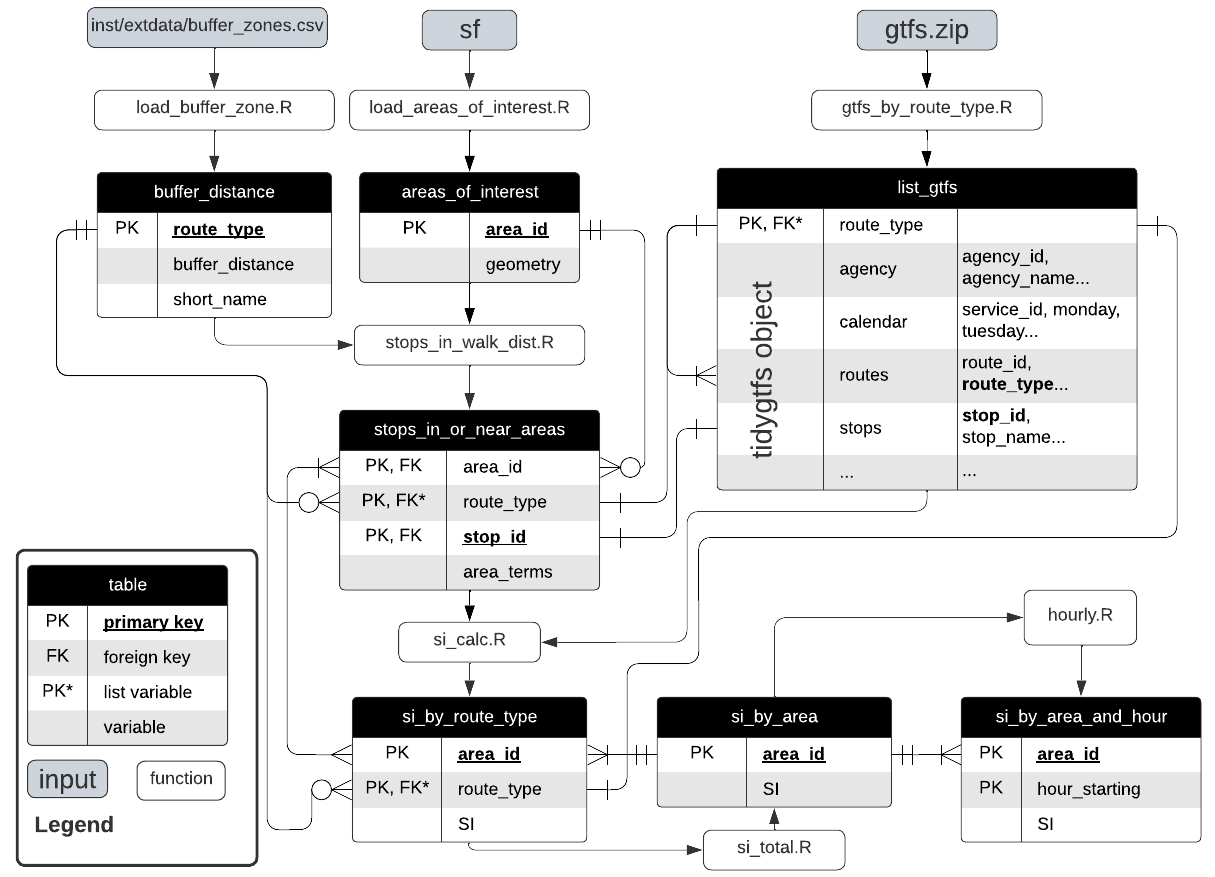
\includegraphics[width=1\linewidth]{graphics/SI_data_structure} \caption{Entity Relationship Diagram (ERD) showing the data structure and functions related to the gtfssupplyindex package}\label{fig:SI_ERD}
\end{figure}

The various functions included in the package and their output are
explained in the following, using the Mornington Peninsula GTFS as a
worked example\footnote{This paper itself was prepared in Rmarkdown and
  is available at
  https://github.com/James-Reynolds/gtfssupplyindex\_main\_paper. Code
  snippets used to produce the outputs of the worked example can be
  viewed there.} Individual steps are as follows:

\begin{enumerate}
\def\labelenumi{(\arabic{enumi})}
\item
  The GTFS data is loaded using\\
  the gtfs\_by\_route\_type function which also splits it into a list
  (by route\_type) of tidygtfs objects, using the
  filter\_by\_route\_type function from the gtfstools package
  \citep{filter_GTFS_by_mode}.
\item
  Geometry information about the areas of interest is loaded by the
  load\_areas\_of\_interest function using the sf package \citep{R-sf}.
  The resultant areas\_of\_interest table
\item
  The walking distance threshold assigned to each route\_type (mode) is
  then loaded, using the load\_buffer\_zone function.
\item
  Stops within the catchment walking distance of each area\_of\_interest
  are then identified using the stops\_in\_walk\_dist function. Figure
  @ref(fig:calculate\_stop\_in\_or\_near\_areas\_verbose) shows how this
  functions identifies the SA1 areas within the 800 metre catchment of
  all three of the Mornington stations.
\end{enumerate}

\begin{figure}
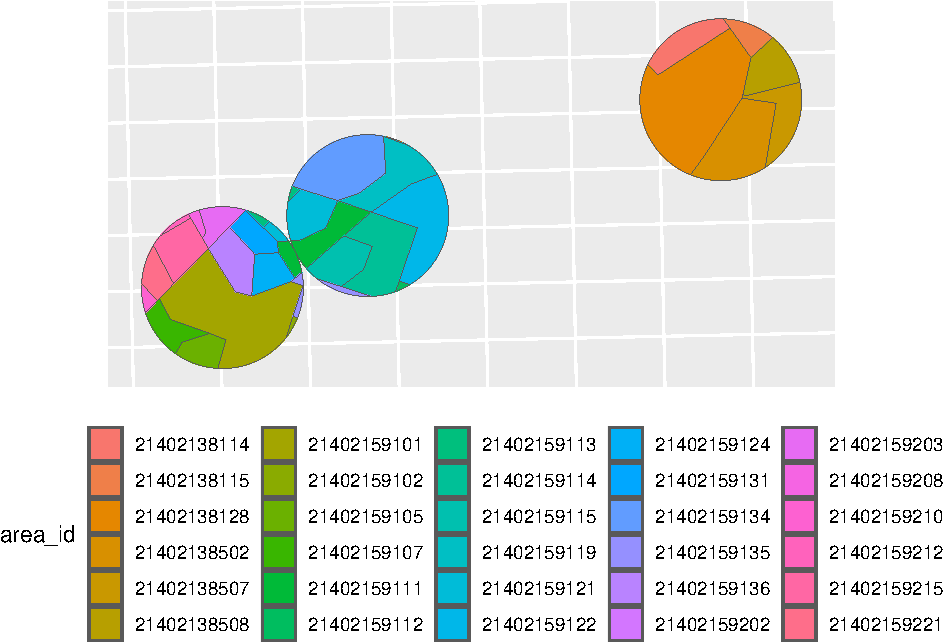
\includegraphics[width=1\linewidth]{Leveraging_GTFS_to_assess_transit_supply_Transport_Geography_files/figure-latex/calculate_stop_in_or_near_areas_verbose-1} \caption{Step 3, stop catchments for the Mornington Penninsula Tourist Railway, showing intersections with SA1 zones}\label{fig:calculate_stop_in_or_near_areas_verbose}
\end{figure}

\begin{enumerate}
\def\labelenumi{(\arabic{enumi})}
\setcounter{enumi}{4}
\tightlist
\item
  SI scores are calculated for a given time period using the si\_calc
  function, which first identifies the number of arrivals in a given
  time period at each stop using code adapted from an article included
  in the tidytransit package \citep{tidytransit_departure_timetable}.
  The area terms of the SI value are calculated, with the si\_total and
  hourly functions providing aggregation by area or by area and hour.
  Figure @ref(fig:SI\_mornington\_20181230\_output) shows the hourly
  output for the Mornington Peninsula Railway, adopting December 30,
  2018 as the date of analysis.
\end{enumerate}

\begin{figure}
\centering
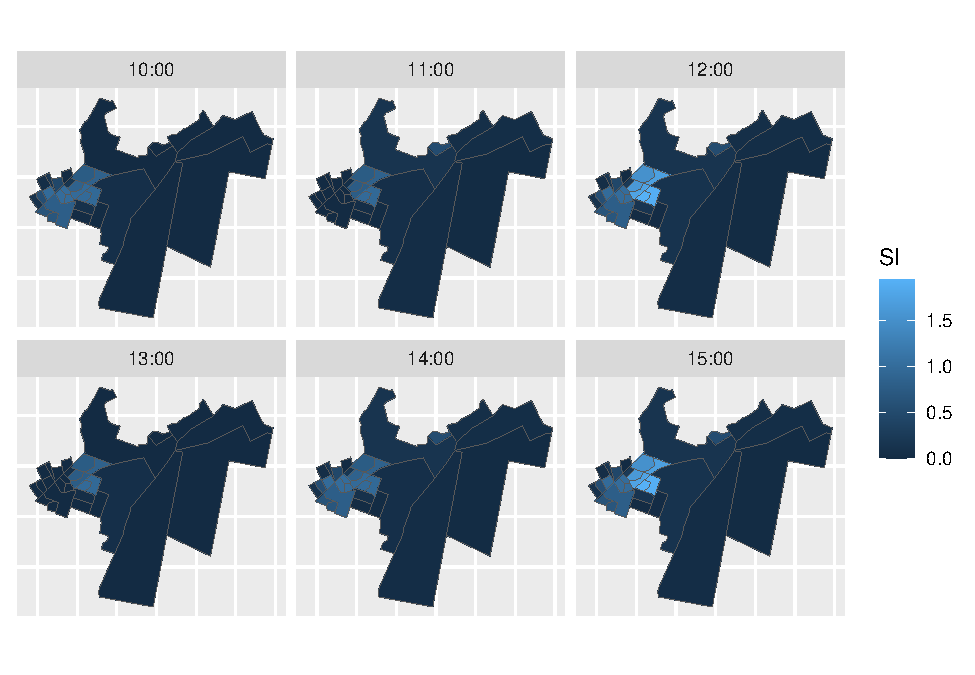
\includegraphics{Leveraging_GTFS_to_assess_transit_supply_Transport_Geography_files/figure-latex/SI_mornington_20181230_output-1.pdf}
\caption{Mornington Penninsula Tourist Railway hourly SI values for
December 30, 2018}
\end{figure}

\subsection{Greater Melbourne}\label{greater-melbourne}

\subsubsection{SI scores}\label{si-scores}

\begin{figure}
\centering
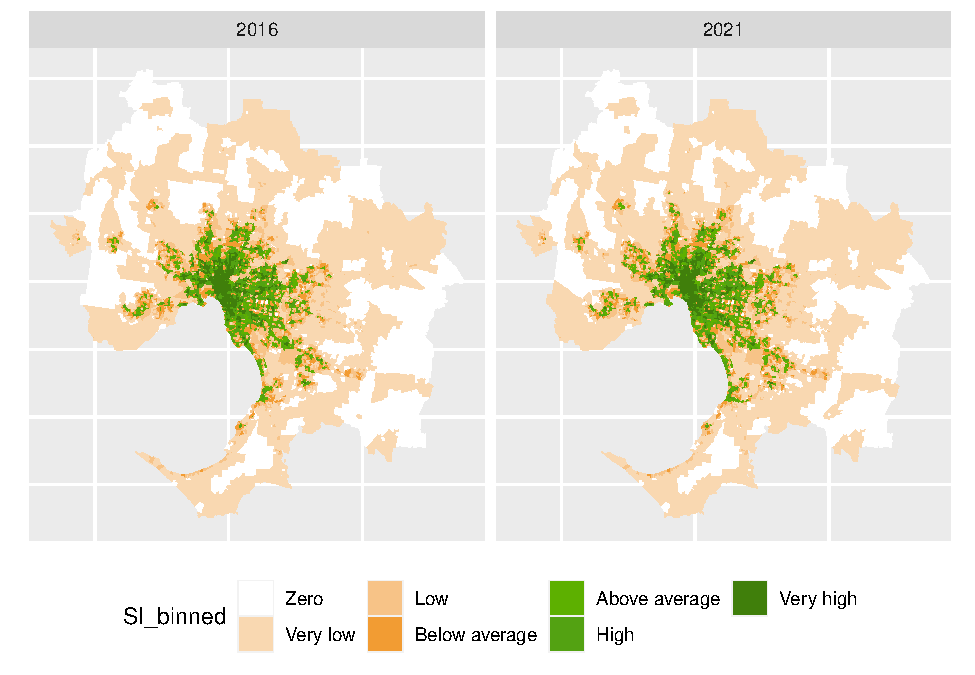
\includegraphics{Leveraging_GTFS_to_assess_transit_supply_Transport_Geography_files/figure-latex/Greater_Melbourne_2016_2021_comparison-1.pdf}
\caption{SI scores, census day 2021}
\end{figure}

\#PICK UP FROM HERE NEED TO ADD SCALE, NORTH ARROW AND INNER, MIDDLE,
OUTER boundaries. CONSIDER ADDING TRAIN LINES AND 2006 GREATER MELBOURNE
BOUNDARY

Figure \ref{fig:Greater_Melbourne_2016_2021} shows SI values on census
day for Greater Melbourne in 2016 and 2021. Comparison to Figure
\ref{fig:Currie_map_SI} indicates that:

\begin{itemize}
\tightlist
\item
  The Greater Melbourne Greater Capital City Statistical Area now covers
  a larger area than it did in 2006, with the northern boundary having
  shifted northwards by up to around 40 kilometres \footnote{See
    https://maps.abs.gov.au/?xmin=15884115.813179802\&ymin=-4689558.173698483\&xmax=16551869.692279067\&ymax=-4397262.977535984\&bottomlayer=ASGS2021:GCCSA\&toplayer=ASGC2006:SD}.
\item
  There are still many areas, typically in the outer parts of Melbourne,
  where there is very low or zero transit supply.
\item
  A similar pattern of higher transit supply near railway lines is
  evident, but there appears to be more areas with above average or
  better service levels further out from the centre of the city.
\item
  In general, above average, high and very high service levels appear to
  be more spread out, especially into the middle suburbs.
\end{itemize}

Comparing 2016 and 2021 suggests that the geographic spread of service
levels has remained largely the same, albeit with some areas that had
little to no transit service appearing to have new services.

\begin{tabular}{l|l|l}
\hline
**Characteristic** & **2016**, N = 10,723 & **2021**, N = 10,999\\
\hline
SI & NA & NA\\
\hline
Mean (SD) & 489 (1,019) & 486 (982)\\
\hline
Median (25\%,75\%) & 229 (92,524) & 237 (95,523)\\
\hline
Range & 0, 15,781 & 0, 15,346\\
\hline
\end{tabular}

\begin{figure}
\centering
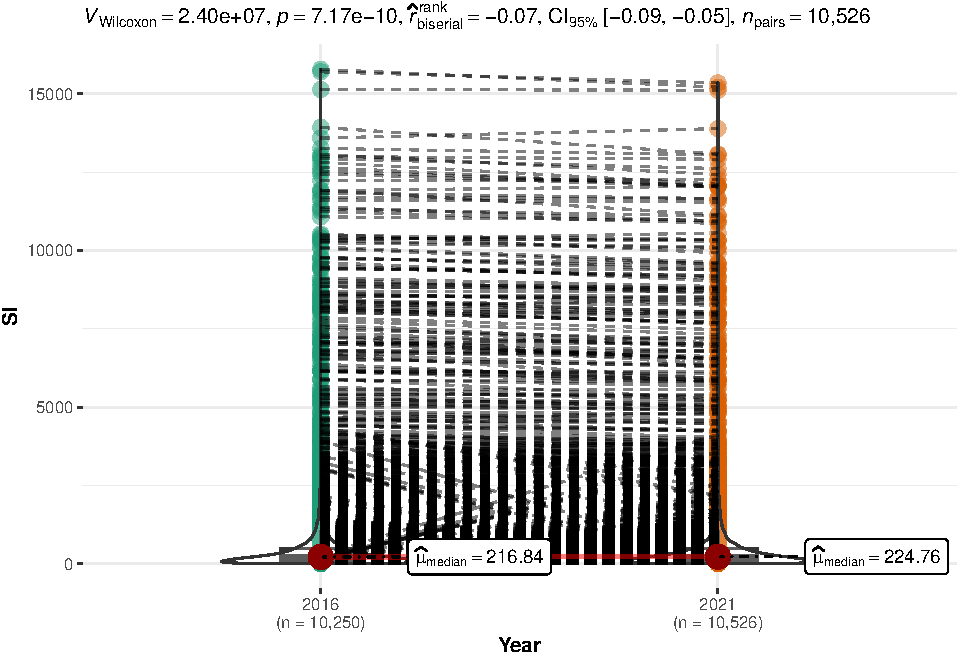
\includegraphics{Leveraging_GTFS_to_assess_transit_supply_Transport_Geography_files/figure-latex/Greater_Melbourne_2016_2021_year_SI-1.pdf}
\caption{SI scores by SA3, census day 2016 and 2021}
\end{figure}

Figure \ref{fig:Greater_Melbourne_2016_2021_year_SI} compares SI scores
for Greater Melbourne across 2016 and 2021. Results indicate a
statistically significant difference, but there does not appear to have
been much change across median, mean, interquartile range or overall
range (See table)

Figure \ref{fig:Greater_Melbourne_2016_2021_scatterplot} compares the
2016 and 2021 SI scores for SA1 zones across Greater Melbourne. Results
indicate a statistically significant relationship, and for most SA1
zones it appears that SI scores have remained largely the same in 2021
as they were in 2016. Of interest, however, may be a group of SA1s that
had SI scores in the range of 3-4,000 in 2016, but only around 2,500 in
2021.

\citet{currie2010identifying} also reported the distribution of SI
scores by category across the number of CCDs and the resident
population.

\begin{table}

\caption{\label{tab:Greater_Melbourne_2016_2021_sa1_population}Distribution of supply index categories, by number of SA1 zones for 2021}
\centering
\begin{tabular}[t]{l|r|l|l}
\hline
SI\_binned & n & percent & valid\_percent\\
\hline
Zero & 0 & 0.0\% & 0.0\%\\
\hline
Very low & 1803 & 16.4\% & 16.4\%\\
\hline
Low & 1794 & 16.3\% & 16.3\%\\
\hline
Below median & 1838 & 16.7\% & 16.7\%\\
\hline
Above median & 1888 & 17.2\% & 17.2\%\\
\hline
High & 1851 & 16.8\% & 16.8\%\\
\hline
Very high & 1821 & 16.6\% & 16.6\%\\
\hline
NA & 4 & 0.0\% & -\\
\hline
Total & 10999 & 100.0\% & 100.0\%\\
\hline
\end{tabular}
\end{table}

\subsubsection{Social needs}\label{social-needs}

Figure \ref{fig:Greater_Melbourne_2021_social_needs} shows the
distribution of categories of social need index scores across Greater
Melbourne for 2021. This figure is analogous to the 2006 value from
\citet{currie2010identifying} shown in Figure \ref{fig:Currie_map_needs}
although, as discussed in the methodology section above, it was not
possible to exactly replicate the \citet{currie2010identifying} approach
as the total number of people within one or more of social need
component groups (necessary to calculate the two relative need
indicators) are not reported in the 2021 census.

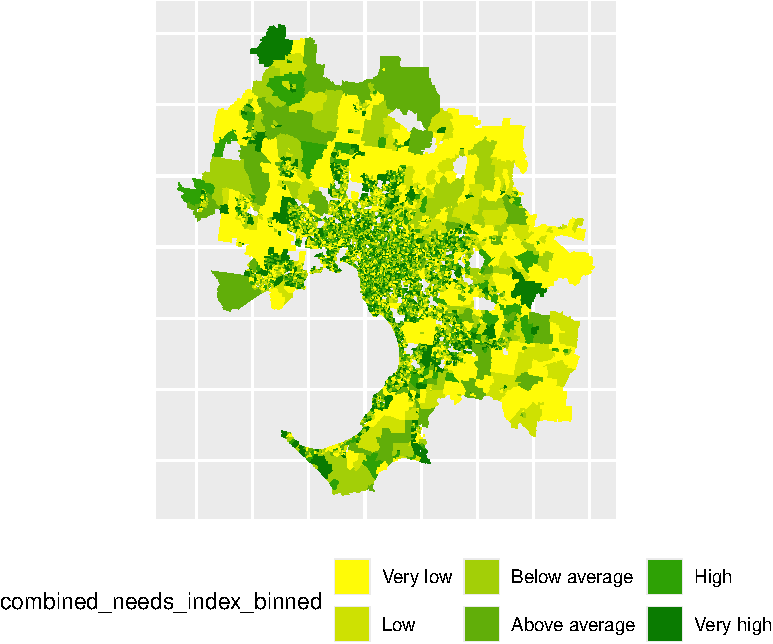
\includegraphics{Leveraging_GTFS_to_assess_transit_supply_Transport_Geography_files/figure-latex/Greater_Melbourne_2021_social_needs-1.pdf}
Figure \ref{fig:Greater_Melbourne_2021_social_needs} appears to indicate
that there is no clear spatial pattern to the distribution of the
categories of the composite need index scores. This appears to contrast
to trend, albeit with some exceptions, towards very high social needs
scores in outer areas identified by \citet{currie2010identifying}
(Figure \ref{fig:Currie_map_needs}). This may, however, be an artifact
of either the differences in the composite needs scores used in this
analysis (due to the lack of data to assess relative needs) compared to
the \citet{currie2010identifying} analysis. As well, the 2021 census SA1
zones generally appear to smalller than the 2006 Census Collection
Districts (CCDs) used in \citet{currie2010identifying}, especially in
outer areas. This will be associated with the growth of Greater
Melbourne's population and spatial dispersment, with many of the large
outer `Very High' CCDs shown in the 2006 map now split into many more
SA1 zones.

\subsubsection{Needs-gap analysis}\label{needs-gap-analysis}

\begin{verbatim}
##  [1] Very high     High          Above average Below average Low          
##  [6] Very low      Very high     High          Above average Below average
## [11] Low           Very low      Very high     High          Above average
## [16] Below average Low           Very low      Very high     High         
## [21] Above average Below average Low           Very low      Very high    
## [26] High          Above average Below average Low           Very low     
## [31] Very high     High          Above average Below average Low          
## [36] Very low      Very high     High          Above average Below average
## [41] Low           Very low      Very high     High          Above average
## [46] Below average Low           Very low      Very high     High         
## [51] Above average Below average Low           Very low      Very high    
## [56] High          Above average Below average Low           Very low     
## [61] Very high     High          Above average Below average Low          
## [66] Very low      Very high     High          Above average Below average
## [71] Low           Very low      Very high     High          Above average
## [76] Below average Low           Very low      Very high     High         
## [81] Above average Below average Low           Very low     
## Levels: Very low Low Below average Above average High Very high
\end{verbatim}

\begin{figure}
\centering
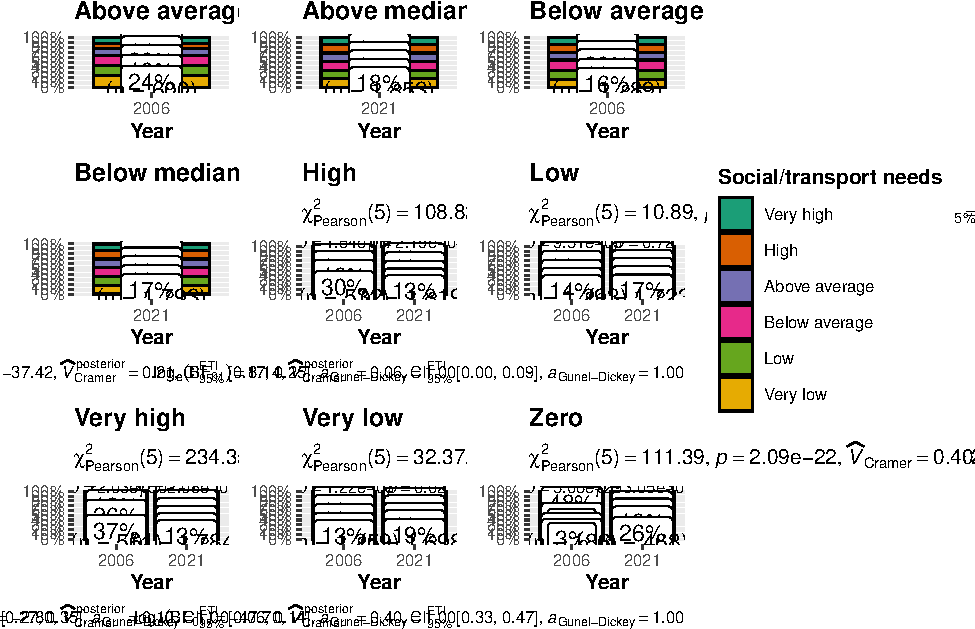
\includegraphics{Leveraging_GTFS_to_assess_transit_supply_Transport_Geography_files/figure-latex/Greater_Melbourne_2006_2021_needs_gap_zones-1.pdf}
\caption{Number of areas by SI and social/transport need category,
comparison between 2006 and 2021}
\end{figure}

\begin{figure}
\centering
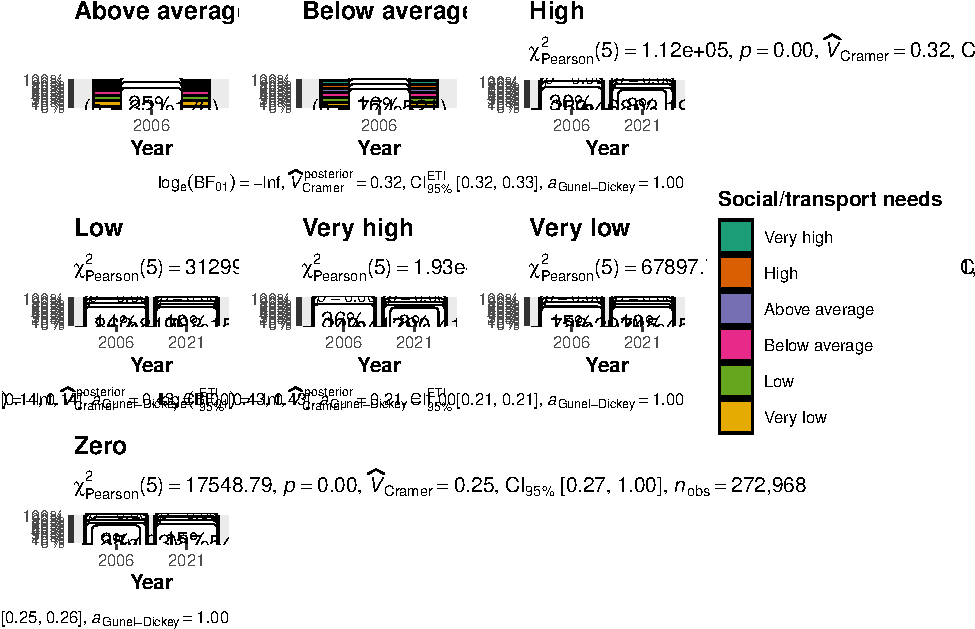
\includegraphics{Leveraging_GTFS_to_assess_transit_supply_Transport_Geography_files/figure-latex/Greater_Melbourne_2006_2021_needs_gap_population-1.pdf}
\caption{Population by SI and social/transport need category, comparison
between 2006 and 2021}
\end{figure}

Figure \ref{fig:Greater_Melbourne_2006_2021_needs_gap_zones} compares
the number of zones\footnote{SA1s in 2021, versus CCD in 2006.} by SI
and social/transport need category between 2006 and 2021. Population is
compared in Figure
\ref{fig:Greater_Melbourne_2006_2021_needs_gap_population}

These results indicate that, in 2021, 66 SA1 zones, (representing
0.6\%of the total 11,138SA1 zones in Greater Melbourne) had no public
transport, but very `very high' social/transport needs. These zones have
a combined population of

\ensuremath{4.5074\times 10^{4}} SA1 zones, representing 45,074(0.9\% of
the total 4,885,773 population) live in areas with no public transport
but have `very high' social/transport needs. This compares to the 89
CCDs (1.6\% of the 5,720 total), representing 37,699 Melbourne residents
(1.1\% of the population) living in areas with no public transport, but
very high social/transport needs reported for 2006 in
\citet{currie2010identifying}.

\subsection{Comparing cases}\label{comparing-cases}

\subsubsection{Population and equality}\label{population-and-equality}

\section{Discussion}\label{discussion}

\subsection{Limitations}\label{limitations}

\subsection{Directions for furture
research}\label{directions-for-furture-research}

\section{Conclusions}\label{conclusions}

\renewcommand\refname{References}
\bibliography{References.bib, packages.bib}


\end{document}
